%  compress using: gs -sDEVICE=pdfwrite -dCompatibilityLevel=1.4 -dNOPAUSE -dQUIET -dBATCH      -sOutputFile=RA-L2016compressed.pdf RA-L2016.pdf
\documentclass[letterpaper, 10 pt, journal, twoside]{IEEEtran}
\IEEEoverridecommandlockouts                              % This command is only needed if 
                                                          % you want to use the \thanks command

%\overrideIEEEmargins                                      % Needed to meet printer requirements.
%\IEEEoverridecommandlockout
%\documentclass[conference]{IEEEtran}
\newcommand{\subparagraph}{}
\usepackage{epsfig,graphicx,cite}
\usepackage{psfrag}
%\usepackage[small,compact]{titlesec}
\usepackage{wrapfig}
\usepackage{mathrsfs}
\usepackage{bm}
\usepackage{cite,url,subfigure,epsfig,graphicx}
\usepackage{verbatim,amsfonts,amsmath,amssymb}
\usepackage{fancyhdr}
\usepackage{mathbbold}
\usepackage{bbm}
\usepackage{mathrsfs}
\usepackage{amsfonts}
\usepackage{cite,url,subfigure,epsfig,graphicx}
\usepackage{amssymb,amsmath,bm,makecell}
\usepackage{indentfirst}
\usepackage{overpic}
\newcommand{\figwid}{0.22\columnwidth}

\usepackage{amsmath}
\usepackage{algorithm}
\usepackage[noend]{algpseudocode}

\usepackage[T1]{fontenc}
\usepackage[utf8]{inputenc}
\usepackage{authblk}



\usepackage{mathtools}
\usepackage[font=footnotesize]{caption}
\usepackage{amsmath}
\usepackage{amssymb}
\usepackage{tabulary}
\usepackage{booktabs}
\usepackage{framed}
\usepackage{fancyhdr}
%\usepackage[hypertex]{hyperref}
\usepackage[hidelinks]{hyperref}
%\IEEEoverridecommandlockouts
\usepackage{cite,url,subfigure,epsfig,graphicx}
\usepackage{times,verbatim,amsfonts,amsmath,color}
%\newtheorem{definition}{\textbf{Definition}}
%\newtheorem{lemma}{\textbf{Lemma}}
%\newtheorem{proof}{\textbf{Proof}}
%\newtheorem{theorem}{\textbf{Theorem}}
%\newtheorem{example}{\textbf{Example}}
%\newtheorem{proposition}{\textbf{Proposition}}
%\newtheorem{remark}{\textbf{Remark}}
%\newtheorem{corrolary}{\textbf{Corrolary}}
%\newtheorem{ex}{\textbf{EX}}
\usepackage{overpic}
\graphicspath{{./},{./pictures/}}
\setcounter{secnumdepth}{4}
\setcounter{tocdepth}{4}
\usepackage[table,xcdraw]{xcolor}
\newcommand{\todo}[1]{ \textcolor{red}{\ttfamily#1}}
\newcommand{\todobox}[1]{\vspace{5 mm}\par \noindent \framebox{\begin{minipage}[c]{0.98 \columnwidth} \ttfamily\flushleft \textcolor{red}{#1}\end{minipage}}\vspace{5 mm}\par}
\let\labelindent\relax \usepackage{enumitem}





\begin{document}
%
% paper title
% can use linebreaks \\ within to get better formatting as desired
\title{A Heterogeneous Robotics Team for Large-Scale Seismic Sensing} 
% Paper headers
\markboth{IEEE Robotics and Automation Letters. Preprint Version. Accepted Jan, 2017}
{Sudarshan \MakeLowercase{\textit{et al.}}: Robotics Team for Seismic Sensing}
% Use only for final RAL version

\author{Srikanth K. V. Sudarshan$^{1}$,
Victor Montano$^{1}$,
An Nguyen$^{1}$,\\ 
Michael McClimans$^{2}$,
Li Chang$^{2}$,
Robert R. Stewart$^{2}$, and
 Aaron T. Becker$^{1}$% <-this % stops a space
 \thanks{Manuscript received: September 10, 2016; Revised November 7, 2016; Accepted January 22, 2017.}%Use only for final RALversion
\thanks{This paper was recommended for publication by Editor Roberts, Jonathan upon evaluation of the Associate Editor and Reviewers' comments. *This work was supported by the National Science Foundation under Grant No.\ \href{http://nsf.gov/awardsearch/showAward?AWD_ID=1553063}{ [IIS-1553063]}.}% <-this % stops a space
\thanks{$^{1}$Department of Electrical and Computer Engineering,}
\thanks{$^{2}$Department of Earth and Atmospheric Sciences,\\ University of Houston, 4800 Calhoun Rd, Houston, TX 77004, USA
        {\tt\small \{skvenkatasudarshan, vjmontano, anguyen43, msmcclimans, lchang13, rrstewart, atbecker\}@uh.edu}}%
\thanks{Digital Object Identifier (DOI): see top of this page.}
}



\maketitle
%\thispagestyle{empty}
%\pagestyle{empty}


\begin{abstract} 
Seismic surveying requires placing a large number of sensors (geophones) in a grid pattern, triggering a seismic event, and recording vibration readings. 
 The goal of the surveying is often to locate subsurface resources.  
Traditional seismic surveying employs human laborers for sensor placement and retrieval. 
The major drawbacks of surveying with human deployment are the high costs and time, and risks to humans due to explosives, terrain, and climatic conditions.
We propose an autonomous, heterogeneous sensor deployment system using unmanned aerial vehicles (UAVs) to deploy mobile and immobile sensors.
The proposed system begins to overcome some of the problems associated with traditional systems.  
This paper provides detailed analysis and comparison with traditional survey techniques. 
Hardware experiments and simulations show promise for automation reducing cost and time. 
 Autonomous aerial systems will have a substantial contribution to make in future seismic surveys. 
\end{abstract}

\begin{IEEEkeywords}
	Aerial Robotics; Robotics in Hazardous Fields; Distributed Robot Systems
\end{IEEEkeywords}

\section{Introduction}\label{sec:Introduction}
% Drop letter for first word of the Introduction
% Here we have the typical use of a "T" for an initial drop letter
% and "HIS" in caps to complete the first word.
% \IEEEPARstart{T}{his} is the first sentence of my Introduction.
% Use only for final RAL version
\IEEEPARstart{s}{eismic} surveying is a geophysical technique involving sensor data collection and signal processing. 
%It aides in identifying hydrocarbon reservoirs such as petrol and natural gas. 
A primary application of the method is in the search for subsurface resources. 
Seismic methods are also used extensively in monitoring natural hazards such as earthquakes. 
Traditional seismic surveying requires manual laborers repeatedly placing geophone sensors at specific locations connected by cables. 
The cable length required is proportional to the area surveyed. 
Surveys routinely cover hundreds of square kilometers, requiring kilometers of cabling. 
Seismic surveying in remote locations is complicated by inaccessibility, harsh  conditions, and  transportation of bulky cables and sensors.  
These factors increase the cost. 

Nodal sensors, a relatively new development in seismic sensing, are autonomous units that do not require bulky cabling. 
They have an internal \emph{seismic recorder}, a micro-controller that records seismic readings from a high-precision accelerometer. 
Because this technology does not require cabling, downtime and overall cost can be reduced. 
However, these sensors are still planted and recovered by hand.  

\begin{figure}
\centering
\begin{overpic}[width=\columnwidth]{intro.pdf}\end{overpic}
\caption{\label{fig:Hetero_overall}
The heterogeneous sensor system presented in this paper: wireless SeismicDarts and a SeismicSpider, both designed for UAV deployment. 
}
\end{figure}

We propose a heterogeneous robotic system for obtaining seismic data, shown in Fig.~\ref{fig:Hetero_overall}. The system consists of two sensors, the SeismicDart and  the SeismicSpider.  
The SeismicDart is a dart-shaped wireless sensor that is planted in the ground when dropped  from an unmanned aerial vehicle (UAV). 
The SeismicSpider is a mobile hexapod with three legs replaced by geophones.
This system is designed to automate sensor deployment, minimizing cost and time while maximizing accuracy, repeatability, and efficiency.
  The technology presented may have wide applicability where quickly deploying sensor assets is essential, including geoscience research~\cite{werner2006deploying}, 
  earthquake~\cite{dominici2012micro} and volcano \cite{nagatani2013volcanic}  monitoring, defense operations~\cite{wu2007efficient}, and wildlife monitoring~\cite{dyo2010evolution,mainwaring2002wireless}. 
  
  
  
  

%
\section[Related Work]{Overview And Related Work}

This chapter presents a \emph{hetoerogenous seismic sensing system}, composed of stand alone geophone nodes deployed from unmanned aerial vehicles {UAV} and autonomous rovers with geophone attached.
We examine experimental data on geophone and soil coupling as a function of drop height and soil type.
We then provide a software tool for analyzing and planning a survey mission's logistic.
Our \emph{heterogenous sensor system} approach is designed to quickly and efficiently perform a survey with minimal manual labor for deployment and collection.

Sudarshan et al. \cite{sudarshan2015using} demonstrated a UAV equiped with four geophone sensors as landing gear.
The UAV in \cite{sudarshan2015using} can fly to a pre-programmed waypoint and land, attaching the geophones to the soil.

The geophones in  \cite{sudarshan2015using} had four problems:
(1) a UAV was required for each additional sensor,
(2) the force for planting the geophone was limited by the weight of the UAV,
(3) the platform required a level landing site,
(4) the magnets in the geophones distort compass readings, causing landing inaccuracy when autonomous.

The \emph{SeismicDart} presented in this system eliminates the need for a seperate UAV per sensor node.
Dropping the SeismicDarts from height also allows for greater penetration, firmer coupling and does not need a level landing site.
The new deployment unit also increase the distance between the SeismicDart's magnet and the UAV's magnetometer unit.

The SeismicSpider, our autonomous rover, can travel to survey locations inaccessible to UAV such as forests, thin atmosphere environments, caves or hard and rocky grounds which SeismicDarts cannot penetrate.
The SeismicSpider can also be deployed by a UAV, as close to the survey node as possible, then move to the desired location.

\subsection{Overview Of Seismic Sensing Theory}

\begin{figure}
	\centering
	\begin{overpic}[width=\columnwidth]{ral2016/Overview.pdf}\end{overpic}
	\caption{\label{fig:sensor_types}
	 Comparing state-of-the-art seismic survey sensors. a.) A traditional cabled system connects geophones in series to a seismic recorder and battery. b.) Autonomous nodal systems give each geophone a seismic recorder and battery.}
	%\vspace{-2em} 
\end{figure}



During seismic surveys, a source generates seismic waves that propagate under the earth's surface. 
These waves are sensed by geophone sensors and recorded for later analysis to detect the presence of resources. 
Fig.~\ref{fig:sensor_types} illustrates the components of current sensors. 

\subsubsection{Geophones}
Magnet-coil geophones contain a permanent magnet on a spring inside a coil. Voltage across the coil is proportional to velocity. 
 Beneath the coil housing is a metal spike. 
  Geophones are \emph{planted} by pushing this metal spike into the ground, which improves coupling with the ground to increase sensitivity. 
 The magnet-coil must be vertical. 
  Misalignment reduces the signal proportional to the cosine of the error.


\subsubsection{Cabled Systems}
Hydrocarbon exploration extensively uses traditional \emph{cabled systems} for seismic data acquisition.
Geophones are connected to each other in series using long cables. This cable is then connected to a seismic recorder and battery. 
The seismic recorder consists of a micro-controller which synchronizes the data acquired with a GPS signal and stores the data onboard. 
This method of data acquisition requires many manual laborers and a substantial expenditure for transporting the cables. 
Rugged terrain makes carrying and placing cables labor intensive, and the local manual labor pool may be unskilled or expensive.
   
\subsubsection{Autonomous Nodal Systems}
\emph{Autonomous nodal systems}~\cite{wood1998distributed} are now being used to conduct seismic surveys.
Unlike traditional cabled systems, autonomous nodal systems are not connected using cables.
The sensor, seismic recorder, and battery are all combined into a single package called a \emph{node} that can autonomously record data as shown in Fig.~\ref{fig:sensor_types}.
Even in these systems the data is generally stored in the onboard memory and can only be acquired after completing the survey.
This delay means errors cannot be detected and rectified while conducting the survey. 
Wireless autonomous nodes are a recent development.
These systems can transmit data wirelessly in real time~\cite{jiang2015geophysical}.
However, these systems still require manual laborers for planting the autonomous nodes at specific locations and deploying the large antennas necessary for wireless communication.
 
\subsection{Related Work}

Seismic surveying is a large industry.
The concept of using robots to place seismic sensors dates to the 1980s, when mobile robots placed seismic sensors on the moon~\cite{LSisMSE81}.
\cite{DSSMaA14} and \cite{coste2013seismic} proposed using a mobile robot for terrestrial geophone placement.
Plans are underway for a swarm of seismic sensors for Mars exploration~\cite{MAPL2006}.
Additionally,~\cite{muyzert2015marine} and~\cite{postel2014drone} proposed marine robots for hydrophone deployment underwater. 
Other work  focuses on data collection, using a UAV to wirelessly collect data from multiple sensors~\cite{wilcox2013seismic}.
Autonomous sensor deployment and mobile wireless sensor networks were studied in~\cite{howard2002mobile,corke2004autonomous,tuna2014autonomous}.
Heterogeneous mobile robotic teams were used for mapping and tracking in~\cite{howard2006experiments}.

%
\section[SeismicDarts]{SeismicDarts}

A SeismicDart combines a geophone (GS-100) with the fins and body of a lawn Jart\textsuperscript{TM}, using a 3D-printed chamber that encloses a WiFi-enabled microcontroller (particle.io Photon\textsuperscript{TM}) as shown in Fig.~\ref{fig:Smart_Dart_overview}. 
The center of the chamber is slotted to fit a wooden plate holding an accelerometer that transmits data wirelessly through the microcontroller. 
The centered accelerometer card allows placing the microcontroller and battery on opposite sides, balancing the dart.
Designs and instructions to build a SeismicDart are available at \cite{Victor2016Thingiverse}.



\begin{figure} \centering
{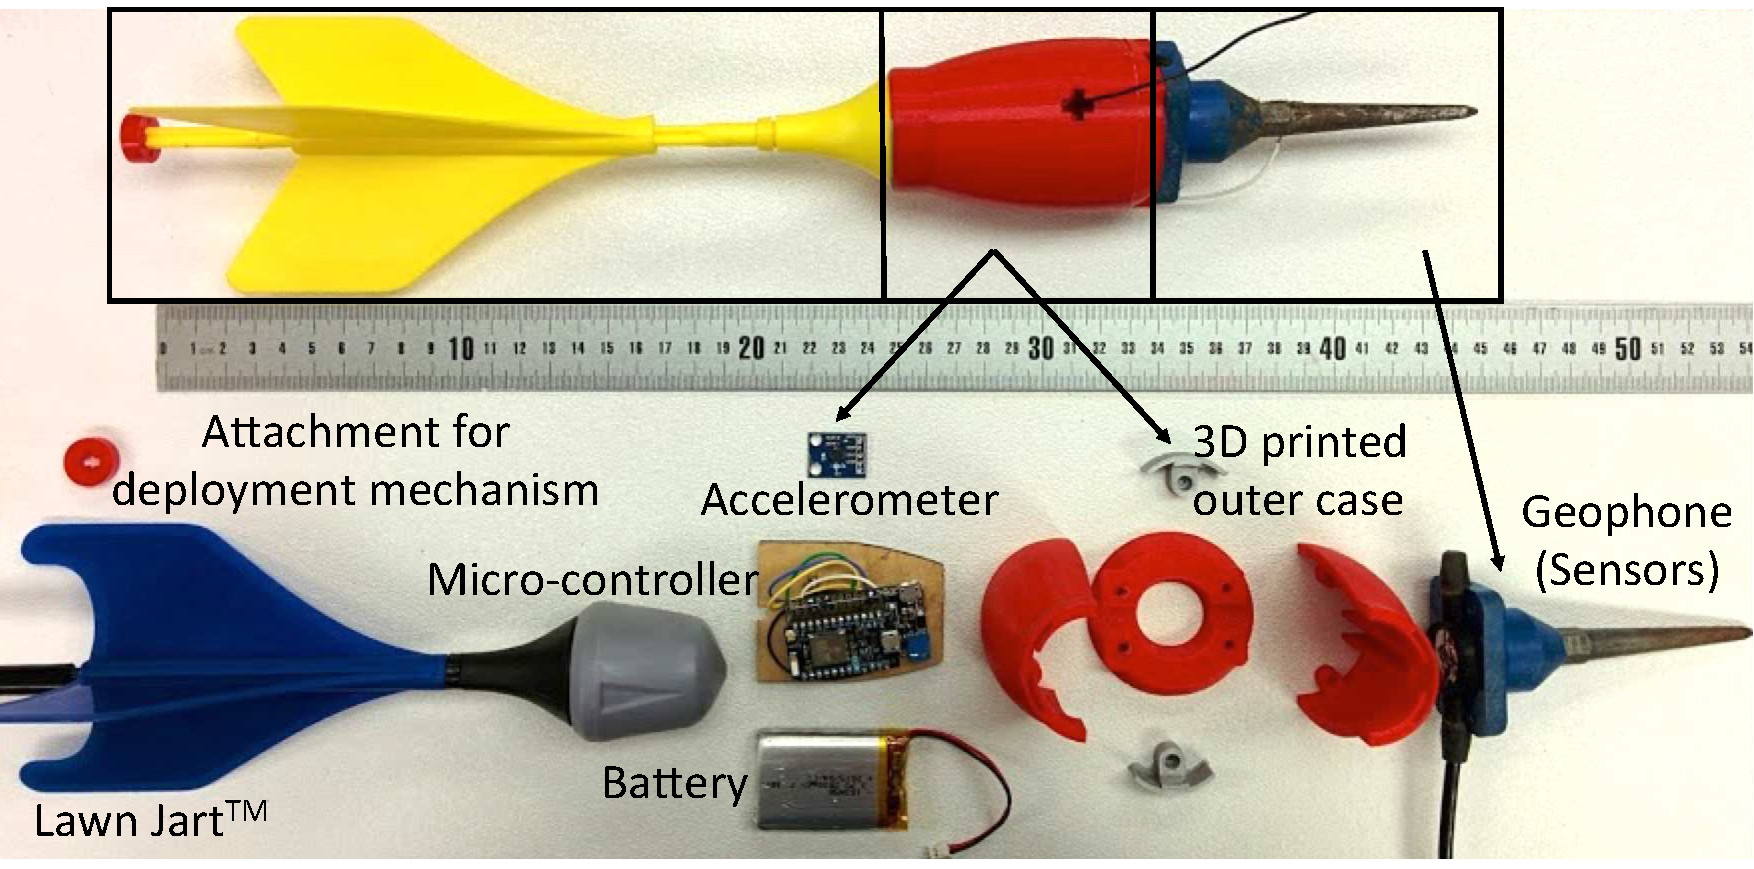
\includegraphics[width=\columnwidth]{ral2016/Smart_Dart_overview.pdf}}
\caption{Components of the SeismicDart sensor: a lawn  Jart\textsuperscript{TM} fin, particle.io Photon\textsuperscript{TM}  micro-controller, 3D printed protective casing, and a geophone.} 
\label{fig:Smart_Dart_overview}
\end{figure}

%%%%%%%%%%%%%%%%%%%%%%%%%%%%%%%%%%%%%%% 
\subsection{Experiments} 
The following sections compare SeismicDart performance.
\subsubsection{ Drop tests in different soils}  


Proper planting of a geophone requires good contact with the soil and the geophone to be in a vertical position. 
Geophone protocol classifies a geophone as well planted if the angle of deviation is less than 10$^\circ$ and the spike has at least 40 mm of penetration.

To determine how SeismicDarts perform in different soils, this experiment measured penetration depth and angle of deviation in seven different soil types as a function of drop height. 
 The soil types were categorized by compression strength, in kg/cm$^2$, measured using a soil pocket penetrometer (CertifiedMTP). Measurements for compression strength vary with a small deviation in measurement location, so we repeated this measurement 10 times at 10 different locations in each soil type and computed the average.
 
 Experiments were conducted using the UAV to autonomously drop a payload of four SeismicDarts at the desired drop height. 
 Tests were conducted at drop heights of 10, 15, 20, and 25 m. 
 We measured the angle of deviation and penetration depth for each drop.
 The angular deviation was measured using two protractors.
 We measured penetration depth by marking where the spike met the soil, pulling the dart from the soil, and measuring the distance from the spike tip to the marking with calipers. 
  We repeated this measurement 12 times for each soil type at each drop height.  The soil compression strengths in these experiments ranged from 0.056 kg/cm$^2$ for river sand, to 4 kg/cm$^2$ for a hard-packed soccer field.

Because the four soil types with the lowest soil compression strength could be well-planted with low drop heights, we performed these tests manually. 
We filled 19 liter (5 gal.) buckets with four soil types and dropped the SeismicDart from six heights.
%Penetration depth and angular deviation were measured. %To measure penetration depth, the buried darts were marked where the spike met the soil, the dart was then pulled from the soil, and the distance from the spike tip to the marking was measured with calipers. The angular deviation was recorded using the accelerometer inside the dart.

 
  % These experiments shows that increasing drop height increases penetration on all soils tested.
  % Also, darts dropped in quiescent air remain vertical if they penetrate the soil.
Experiment results plotting penetration depth as a function of drop height are displayed in Fig.~\ref{fig:DepthPlotIndoors}, and angle of deviation as a function of drop height in Fig.~\ref{fig:AnglePlotIndoors}.   Both graphs are annotated with values for soil compression strength. 

\begin{figure} \centering
{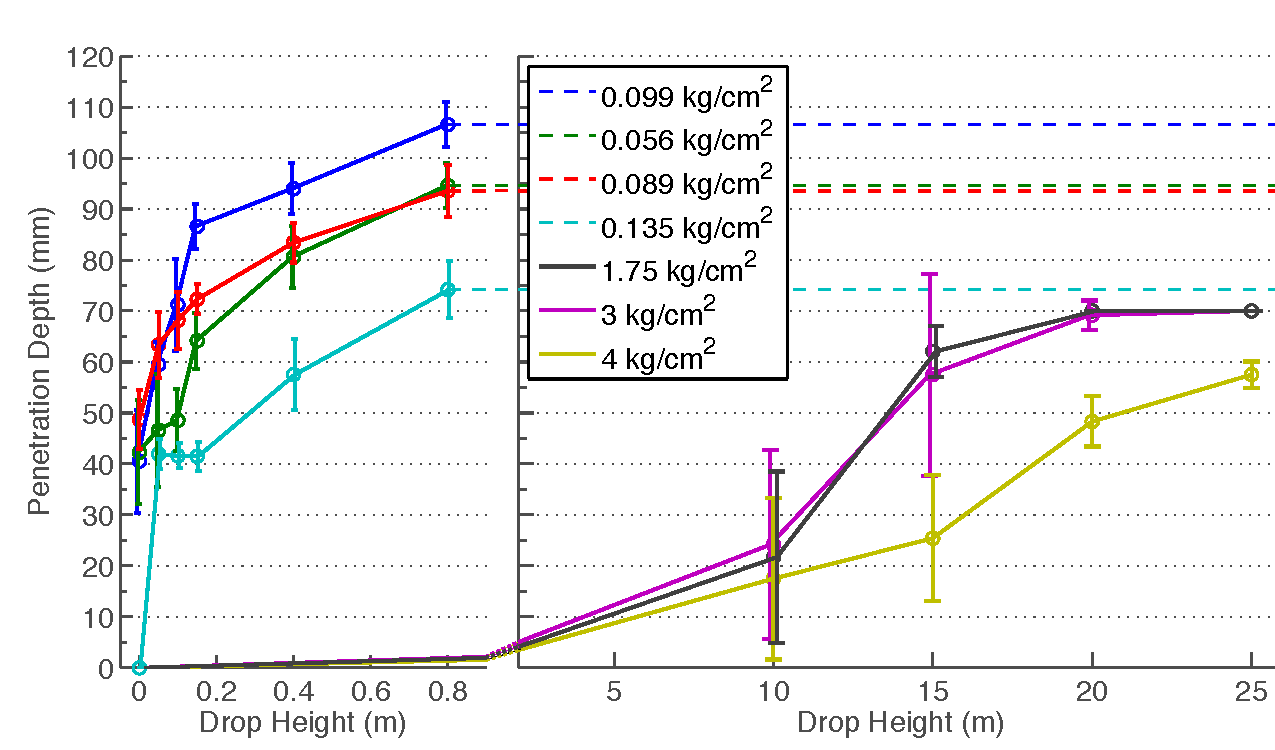
\includegraphics[width=\columnwidth]{ral2016/AutoPenetrationDepth2.pdf}}
\caption{Drop height vs. penetration depth in seven soil types. Drops were performed autonomously and each data point represents 12 trials. Increasing the drop height increased the penetration depth for all seven soil types.} 
\label{fig:DepthPlotIndoors}
\end{figure}

\begin{figure} \centering
{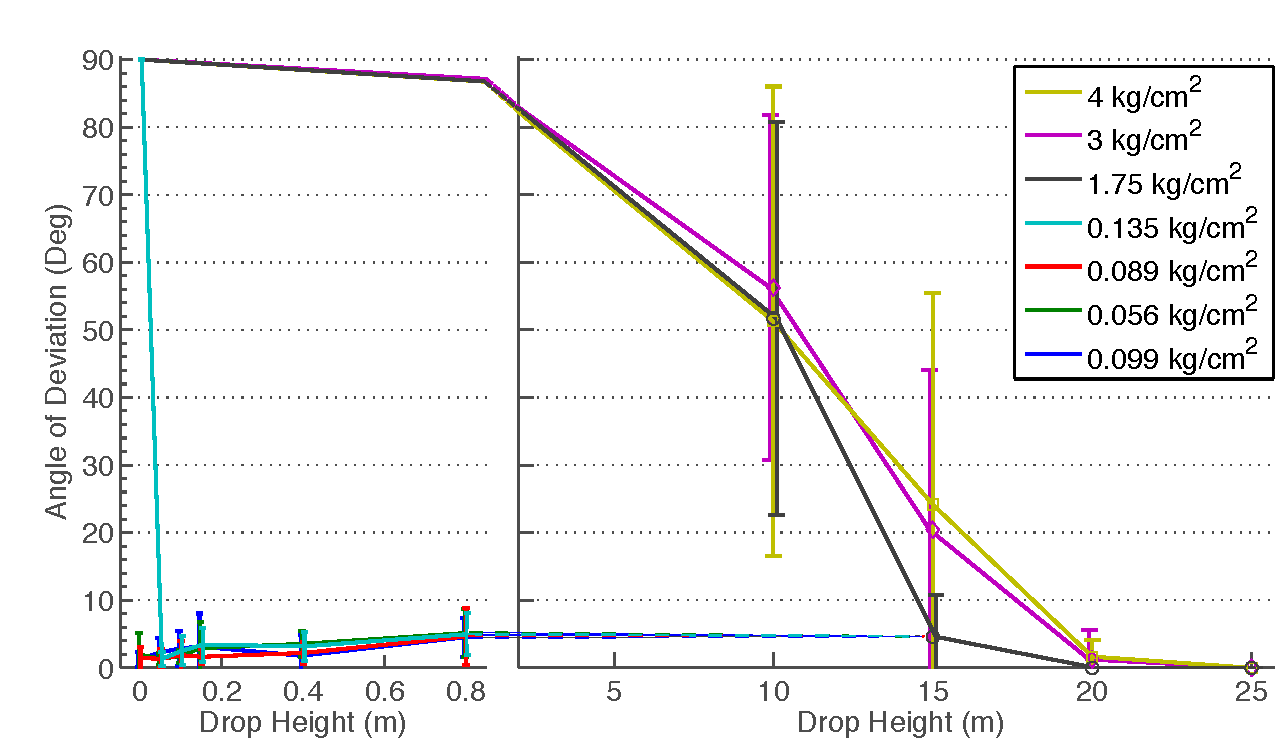
\includegraphics[width=\columnwidth]{ral2016/AutoPenetrationAngle2.pdf}}
\caption{Drop height vs. angle of deviation in seven soil types. Drops were performed autonomously and each data point represents 12 trials. Increasing the drop height reduced the angle of deviation for all seven soil types.} 
\label{fig:AnglePlotIndoors}
\vspace{-1em}
\end{figure}

If a SeismicDart is dropped from a sufficient height into penetrable soil, the spike will be buried into the soil and the geophone will have a small angular deviation from vertical. Soils with higher compression strength require higher drop heights. Error bars show that variance decreases with drop height for angle of deviation and penetration depth.  
 All drops from heights 20 m or more achieved the goals of an angle of deviation less than 10$^\circ$ and at least 40 mm of penetration.   

The autonomous tests were conducted with 16 km/hr winds, demonstrating that drop heights 20 m or higher were sufficient to counter disturbances from the wind. %https://www.windfinder.com/forecast/galveston_airport

\subsubsection{Shot gather comparison} 
Geophysical explorationists often use thousands of geophones to conduct a seismic survey. 
 As a proof-of-concept, this experiment ran a small-scale seismic survey to compare the performance of a traditional cabled four geophone system with readings from four autonomously deployed SeismicDarts.
Flying autonomously at a drop height of 25 m, the UAV flew to GPS waypoints spaced 4 m apart and deployed one dart at each location. 
A seismic survey technician manually planted four traditional cabled geophones, each 10 cm from a deployed SeismicDart. 
A seismic wave was generated using a sledgehammer hitting a steel plate.

Results of the field test comparison between the traditional cabled geophone system and the SeismicDarts are shown in Fig.~\ref{fig:shotgather_auto_drop}.   
Data were obtained using a \emph{StrataVisor}, a device that can obtain, store, and plot the sensed data. 
The \emph{StrataVisor} is extensively used with traditional geophone setups because the geophones can only sense vibrational waves and are dependent on other devices for storage and data processing. 
To allow a fair comparison with geophones, the SeismicDart's  ability to store sensed data was not used in this experiment. 
 The \emph{StrataVisor} records the geophone voltage at 2000 Hz, using a 24 bit ADC.

The readings from both systems are qualitatively similar, with no discernible phase or amplitude differences. Let $X$ be measurements from the traditional geophone and $Y$ the corresponding voltages from a SmartDart.
The percent peak-to-peak error and normalized root-mean-square error (NRMSE) are defined as
\begin{align}
e_{pp} &= 100 \left( \frac{ \max(X) - \min(X) }{ \max(Y) - \min(Y) } -1\right) \\
  \text{NRMSE} &=\frac{100}{\max(X) - \min(X)} \sqrt{ \frac{ \sum_{i=1}^n \left( X_i - Y_i \right)}{n} }.
\end{align}
The peak-to-peak errors were [-6.33, -1.15, -1.81,  9.84] \% for sensors at [4,8,12,16] m from the source.
 The NRMSE were [1.05,1.27,3.98,4.39] \% for sensors at [4,8,12,16] m from the source.
%$e_{\text{4 m}}  =  -6.3 \%, e_{\text{8 m}}  =  11.93 \%, e_{\text{12 m}}  = -1.81\%, e_{\text{16 m}}  = 0.981 \%$. 
%The RMSD error were $RMSD_{\text{4 m}}  =  -6.3 \%, RMSD_{\text{8 m}}  =  11.93 \%, RMSD_{\text{12 m}}  = \%, RMSD_{\text{16 m}}  = 0.981 \%$. 
Readings were also compared using a Pearson product-moment correlation coefficient, which gives a correlation measurement between $-1$ and $+1$ where $+1$ is total positive linear correlation:
\begin{align}
\rho_{X,Y} = \frac{E\left[  (X-\mu_X) (Y-\mu_Y)  \right]}{  \sigma_X, \sigma_Y}.
\end{align}

The correlation coefficients were $\rho_{\text{4 m}}  =  0.9813, \rho_{\text{8 m}}  =  0.9836, \rho_{\text{12 m}}  =  0.8600, \rho_{\text{16 m}}  = 0.8114$. These correlations decrease with distance. The SeismicDart is subject to low-amplitude noise, which is easiest to see in the fourth sensor because it was 16 m from the seismic source and thus had the lowest signal amplitude.  This noise is potentially due to wind striking the SeismicDart's fin. The effect of noise can be mitigated by using larger seismic sources such as a vibration truck or explosives.



\begin{figure} \centering
  {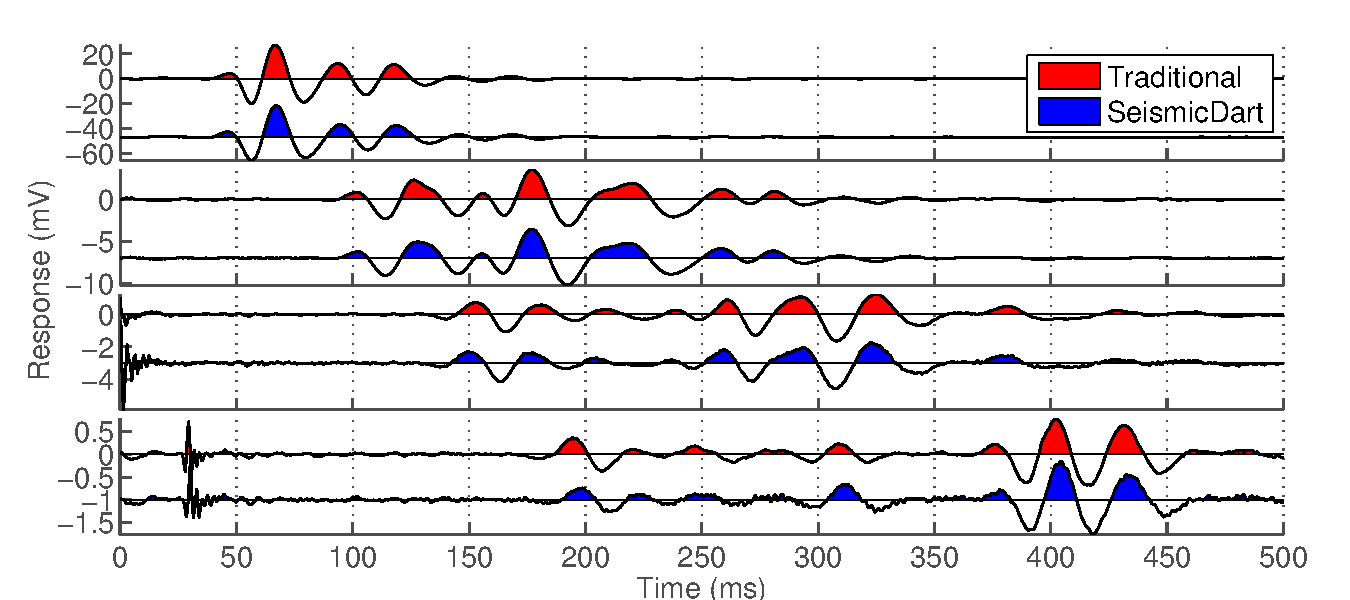
\includegraphics[width=\columnwidth]{ral2016/SeismicSurveyComparison.pdf}}
 \caption{Raw voltage data from shot gather comparison of four traditional geophones and four autonomously dropped SeismicDart sensors.  
 \label{fig:shotgather_auto_drop}}
\end{figure}

\subsection{SeismicDart Deployment and Retrieval}
First, the SeismicDarts are loaded onto to a UAV. 
Currently, a maximum of four sensors can be dropped in a single flight. 
The flight plan communicated to the UAV provides a GPS waypoint for each SmartDart. 
The UAV flies to and drops a SmartDart at each waypoint, then returns home. 

Deployment is only one part of a survey. Large surveys require moving and reusing sensors.  
Because SmartDarts are more expensive than standard geophones, rapid reuse is essential.
The UAV has an underslung hook for picking up a SeismicDart.
Retrieval is facilitated by attaching a wire loop to the SeismicDart tail.
 This loop provides a target 300 mm in diameter for the hook, yet still allows autonomous deployment, as shown in Fig.~\ref{fig:SeismicDart_DR}.
Currently, retrieval is performed by manually piloting the UAV, but the loop size is within the accuracy of a UAV equipped with RTK GPS.
%Automating retrieval is out of the scope of this paper.



\begin{figure} \centering
  {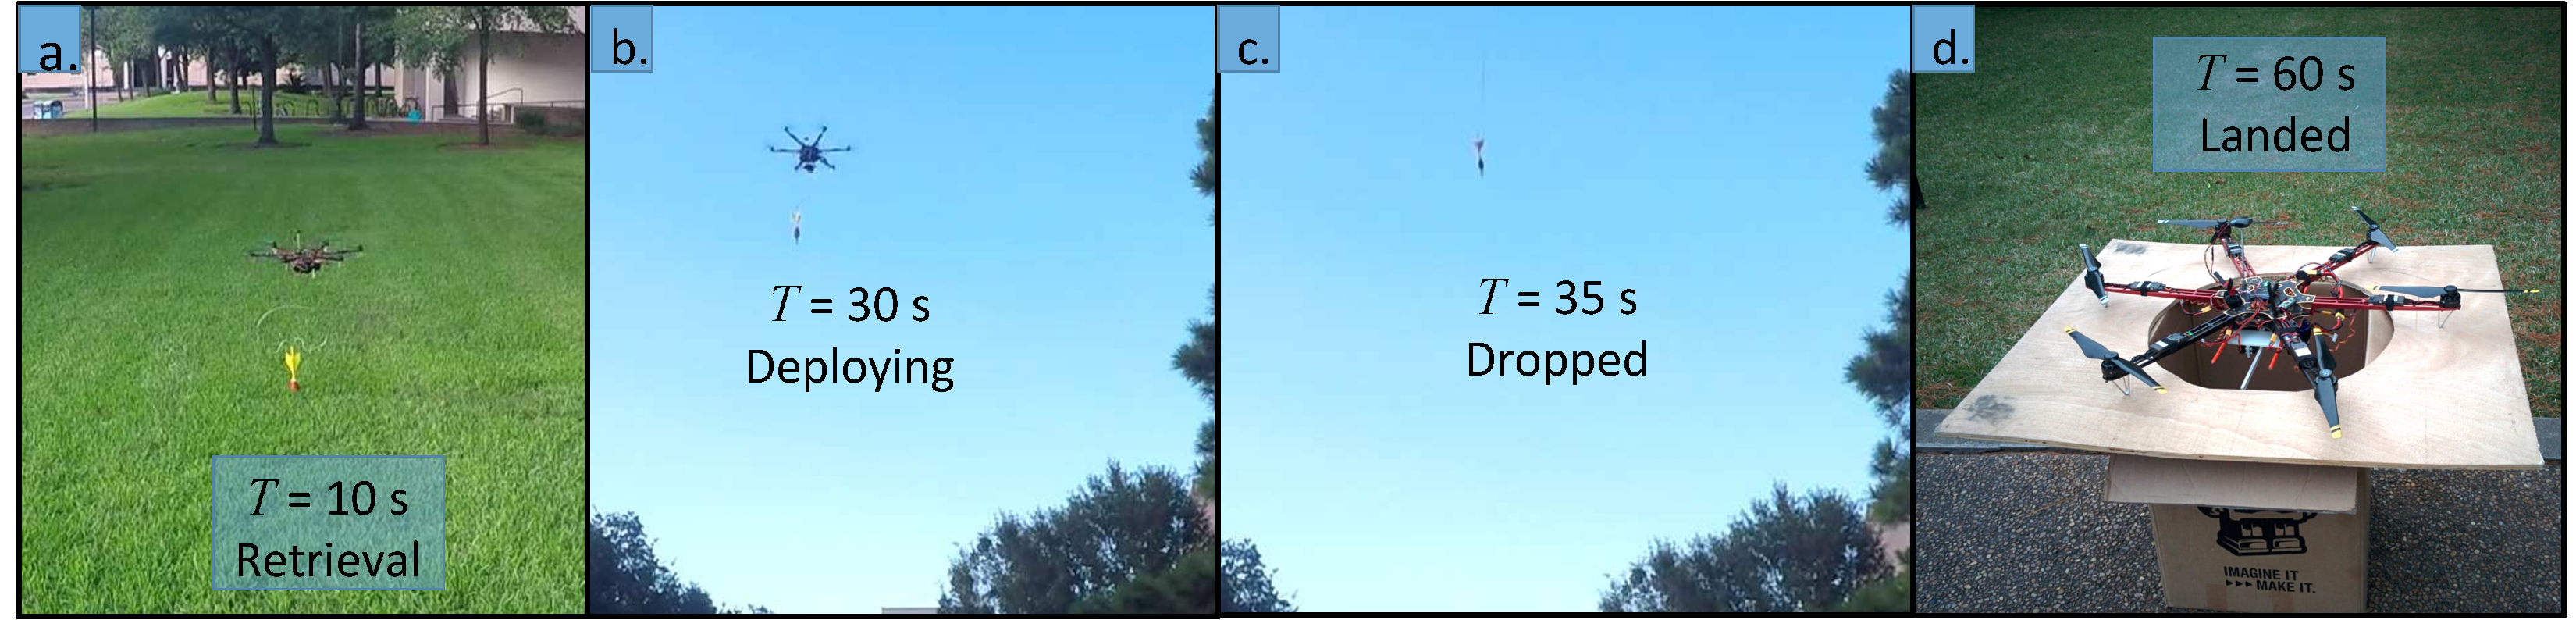
\includegraphics[width=\columnwidth]{ral2016/SeismicDart_DR.pdf}}
 \caption{SmartDart retrieval and redeployment.  See video attachment. 
 \label{fig:SeismicDart_DR}}
\end{figure}
 

%
\section{SeismicSpider}\label{sec:SeismicSpider}


\begin{figure} \centering
  {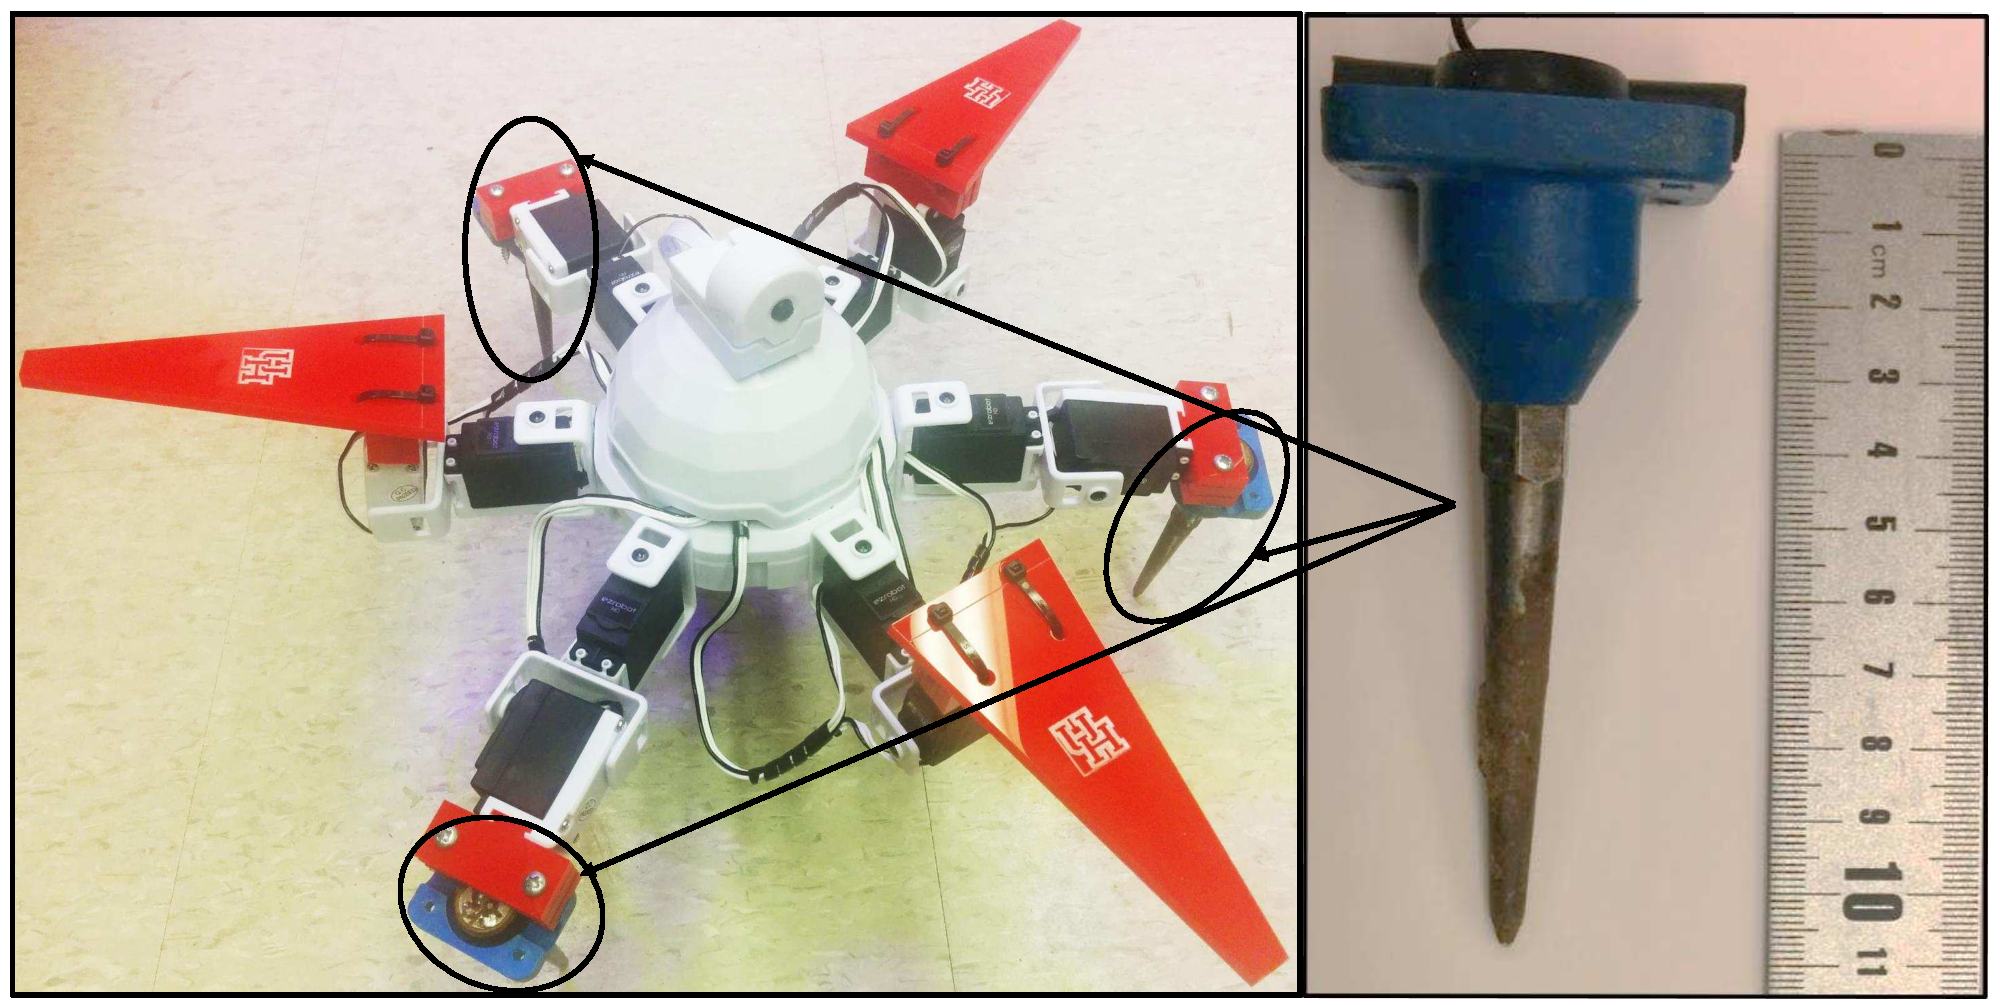
\includegraphics[width=\columnwidth]{Hex_overview.pdf}}
 \caption{The SeismicSpider is a six-legged mobile robot where geophones replace three legs. It is drone deployable, can sense and record seismic data, and can move to desired locations, including terrain the SeismicDart cannot access.} 
 \label{fig:Hex_overview}
\end{figure}


The SeismicSpider, shown in Fig.~\ref{fig:Hex_overview}, is built from the Six Hexapod kit designed by EZ-Robots. Each of the six legs is powered by two 15 kg$\cdot$cm lever servos. Three legs were replaced by three GS-20DM 14 Hz geophones from Geospace Technologies. The remaining three legs were designed to match the geophone dimensions.

 Our initial plan to use three geophones required the spider to raise the three inactive legs while acquiring data. This lack of support caused excessive strain on the three servo motors responsible for holding the spider upright, introducing unwanted vibration into the system.  Positioning the geophone legs at 20$^\circ$ to normal enhances stability and relieves the excessive stress on the servos. 
 The three geophones were in series, so with each geophone leg angled inward, superposition replicates the signal from one vertical geophone.
 
 Traditional geophones are mounted in an insulated, shock-resistive enclosure on a spike. The spikes, varying in length, are inserted into the ground to ensure a firm coupling with the environment. The design of our SeismicSpider prevents full depth insertion of the 88 mm spikes. 

	To overcome the coupling issue we are using three geophones per station compared to the typical one. Our immediate goals were to compare amplitude response to that of a standard single station.	
 

\subsection{Shot gather comparison}
%\subsubsection{Accuracy plot}
%Hexapod move to desired GPS location  (plot accuracy)\\
%\subsubsection{ Shot gather comparison}

A line of twenty-four geophones (GS-20DM 14 Hz) were laid out at one-meter intervals with our inline source seven meters from the nearest geophone. Beginning from the farthest offset of 31 m we manually aligned the Spider with the corresponding geophone, fired the source, then moved one meter ahead. 

%\paragraph{Results}
Data from the shot gather comparison is shown in Fig.~\ref{fig:shotgatherHexpod}.
The response for three geophones in series was 5 dB greater than a single geophone. The geophone wires proved insufficient to insulate against 60 Hz noise. Hence the raw data from the traditional setup as well as the SeismicSpider was processed with a (3-50) band-pass filter. Finally, the SeismicSpider data was attenuated by $-5$dB to level the comparison.    

\begin{figure} \centering
  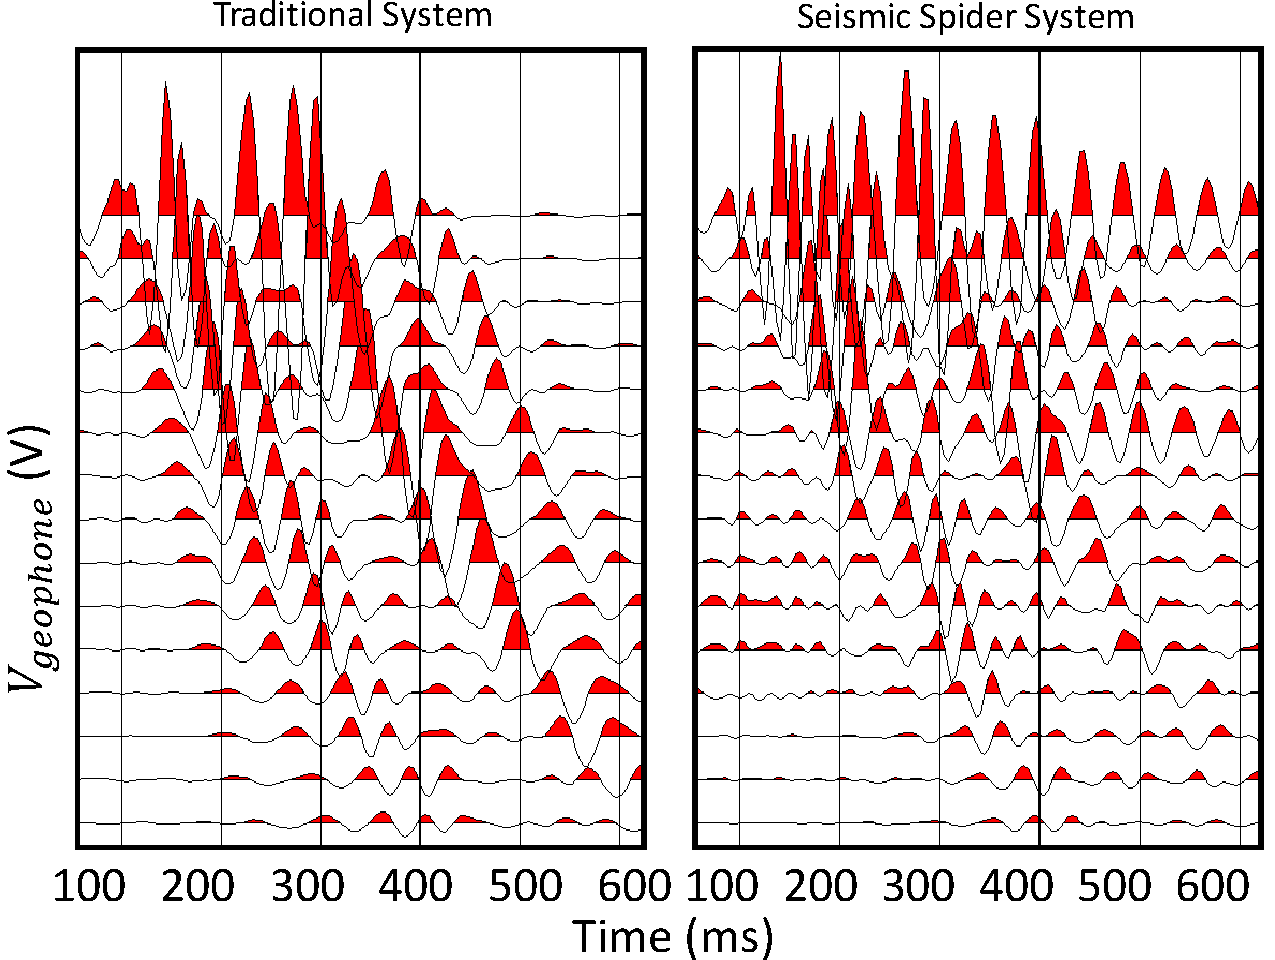
\includegraphics[width=\columnwidth]{shotgather_hex.pdf}
 \caption{Shot gather comparison of traditional geophones vs. SeismicSpider. 
 \label{fig:shotgatherHexpod}}
\end{figure}

%\paragraph{Future work}	we must filter 60 Hz noise, compare adding geophones to all six legs, and design a larger seismic survey to ensure adequate data for phase analysis. Design improvements could be done to make the SeismicSpider an active sensor.   


\subsection{Deploying and Retrieving the SeismicSpider}

\begin{figure} \centering
  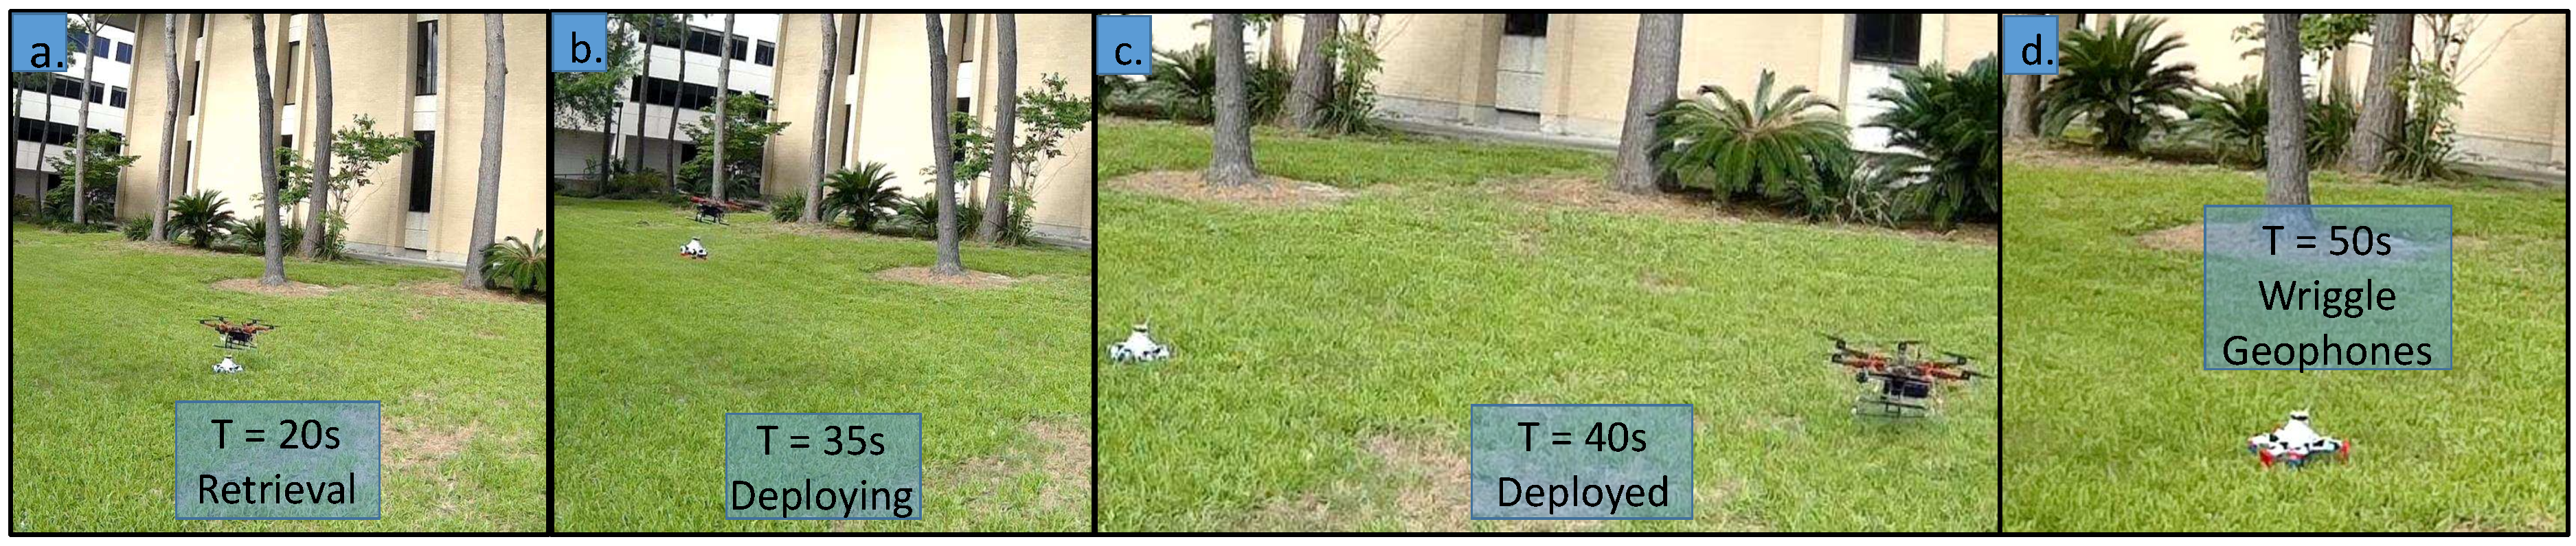
\includegraphics[width=\columnwidth]{SeismicSpider_DR.pdf}
 \caption{SeismicSpider retrieval and redeployment. See video attachment. 
 \label{fig:SeismicSpiderDR}}
\end{figure}

The UAV's purpose is to deploy sensors at desired GPS waypoint locations. The SeismicSpider is a mobile robot, but it is substantially slower than the UAV.  The UAV carrying the SeismicSpider flew autonomously to a programmed waypoint. The deployment mechanism included a hook controlled by a servo attached to the UAV. The UAV lowered to a waypoint 0.5 m from the ground, then the servo was triggered to unhook the SeismicSpider.  The SeismicSpider was then wirelessly powered on. 
The SeismicSpider also has an onboard GPS, enabling it to navigate to desired waypoints. 
After walking to the sensing location, the SeismicSpider was programmed to shake its three non-sensing legs to plant its geophone legs into the ground.  
  Currently, autonomous deployment of sensors is implemented, but the retrieval is piloted. 
Combining the mobility of the SeismicSpider with the speed of the UAV enables reaching locations inaccessible by air or impossible to penetrate by SmartDarts.
Fig.~\ref{fig:SeismicSpiderDR} shows the SeismicSpider being retrieved and then redeployed by a UAV.






%
\section{UAV and deployment unit}\label{sec:DeploymentUnit(UAV)}

The UAV is a custom-built, 1.77 m wingspan hexacopter, controlled by a Pixhawk flight controller running ArduPilot Mega flight software. The UAV has a 3DR GPS module using the UBlox NEO-7 chipset.


 The deployment mechanism allows the UAV to carry four SeismicDarts in a circular array, and release them when it reaches the desired GPS location, one at a time.
 The rear of the dart has a circular tip that locks into the deployment mechanism, and rests on a rectangular slot-path. 
 A servomotor rotates the dart tips through the rectangular slot-path, allowing darts to release from a circular opening,  as shown in Fig.~\ref{fig:deployment_system}.



\begin{figure} \centering
  {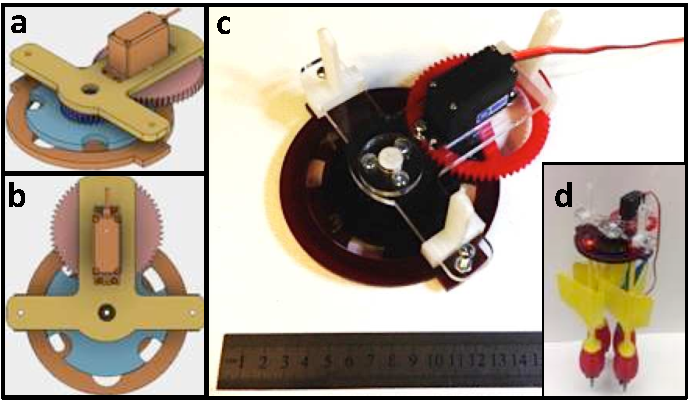
\includegraphics[width=\columnwidth]{deployment_system.pdf}}
 \caption{Deployment system for dropping SeismicDarts from the UAV. Pictured design holds four darts, but can be scaled according to the UAV's carrying capacity.} 
 \label{fig:deployment_system}
\end{figure}




\subsection{Autonomous drop demonstration and accuracy}

The current UAV can place a SeismicDart within $\pm1$ m of the desired location.  
This range is within tolerances for seismic surveys because often features (rocks, water, etc.) exist that require this amount of error from theoretically assigned locations and some survey designs include a random placement component to improve noise cancellation.
%(3) this error minimally perturbs the data since seismic waves travel at 600 m/s near the surface, so a one-meter inaccuracy equates to $\approx$1.6 ms delay.
%(4) the response of a receiver to seismic vibrations is an average over a number of meters.  ?? what does this mean??

To accurately perform a seismic survey, the sensors do not need to placed accurately, but their position must be known within $\approx$ 0.01 m. 
 Knowledge of the exact location compensates for placement inaccuracy.
 Localization can be achieved by placing an RTK GPS in each dart.  A lower-cost solution would use an RTK GPS on the SeismicDrone and perform image registration with the downward facing camera.  As shown in the multimedia attachment, even at a 25 m drop height a planted dart occupies dozens of pixels, enabling cm-level localization accuracy.


%allows corrections for jitter in signal arrival times due to  placement inaccuracy.


%Exp 4: Automatic drop from drone, accuracy in placement
\begin{figure} \centering
  {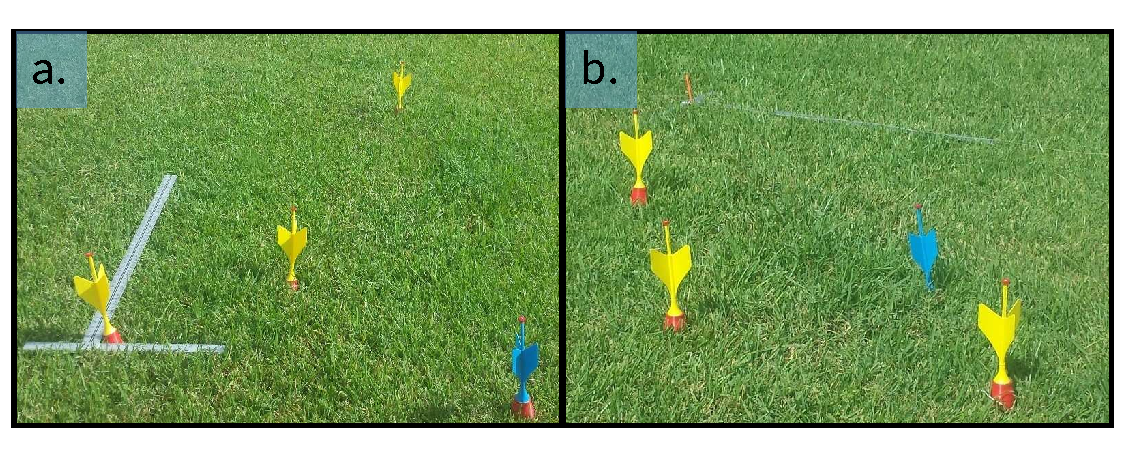
\includegraphics[width=\columnwidth]{accuracy_test_overview.pdf}}
 \caption{a.) First set of darts with reference axes. b.) Third dart set. } 
 \label{fig:Accu_test_darts}
\end{figure}

For the accuracy test, six sets of darts, four darts in each set, were dropped on the same GPS waypoint. Between each drop, the UAV traveled to a nearby GPS waypoint to cancel out the flight controller's stable hover.
The UAV then returned to the launch platform to be reloaded, we recorded the dart landing positions, collected the darts, and reloaded the darts on the UAV for the next deployment set.
The measurement method of the darts' positions are shown in Fig.~\ref{fig:Accu_test_darts}.
Results are shown in Fig.~\ref{fig:SD_accu.pdf}.
  
%To measure position, one dart was picked from the first set as the reference point (the lower left in Fig.~\ref{fig:Accu_test_darts}b), hence the first data point was (0,0). A 1-m T-square was placed with the origin at the dart's drop point to establish reference axes.


 %A rod was placed in the position of the first dart to keep reference as shown in Fig.~\ref{fig:Accu_test_darts}c. 
% The T-square was kept in place and mason twine was suspended to lengthen the reference axes. 
% Future deployments were measured  using the reference point and axes. 



\begin{figure} \centering
  {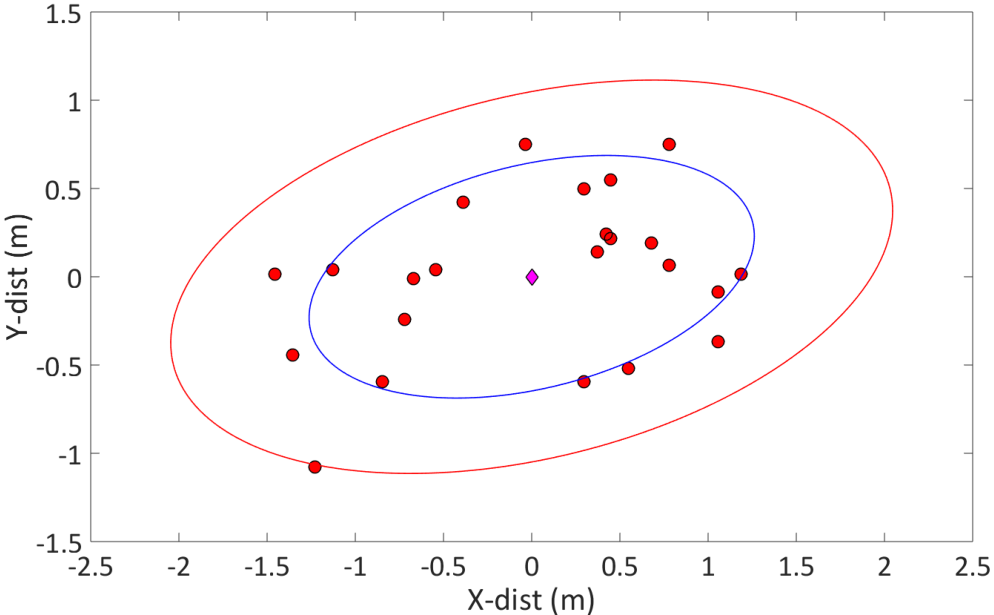
\includegraphics[width=\columnwidth]{SD_accu.pdf}}
 \caption{Targeting accuracy.  Circles show landing locations of 24 darts, each commanded to drop at the same GPS location. The mean position is marked by a diamond, ellipses show  $\sigma$ and 2$\sigma$ covariance.
 \label{fig:SD_accu.pdf}}
\end{figure}


\subsection{Height vs. penetration depth}
%Exp 5: Height vs. penetration depth

FAA rules require that UAVs fly below 400 feet (122 m). Our highest drop tests were from 25 m, and resulted in well-planted geophones on a compacted field with density 4 kg/cm$^2$. Harder soils may require faster impact velocity, so this section examines possible impact velocities as a function of drop height.
For ease of analysis, we will assume the SeismicDart has a constant coefficient of drag $C_d$ and that the drag force is proportional to velocity squared and equal to $\frac{1}{2} v^2 \rho A C_d$, where $v$ is the velocity, $A$ the cross-sectional area and $\rho$ the density of air.  
 The tests were performed near sea level, so $\rho \approx 1.225~\text{kg/m}^3$.
  The dart body is 0.06 m in diameter so $A=0.028$ m$^2$.  We will assume the dart $C_d$ is between that of a streamlined body $C_d=0.04$ and that of an arrow $C_d=1.5$~\cite{miyazaki2013aerodynamic}, and choose that of a sphere $C_d=0.47$.
The terminal velocity is then
\begin{align}
v_T = \sqrt{\frac{2 m g}{\rho A  C_d}} \approx 59 \text{ m/s.}
\end{align}
The velocity at impact is a function of the drop height $h$.
\begin{align}
v_{impact} = v_T  \sqrt{ 1 - e^{ -\frac{\rho A  C_d}{m} h }} \approx 59\sqrt{ 1 - e^{ -0.008 h }} \text{ m/s}
\end{align}
With  $C_d=0.47$, our drop from 25 m achieves only 43\% the terminal velocity (21.1 m/s), and for $C_d=0.04$ only 13\% terminal velocity  (22.0 m/s).
%This implies our tests are far from the limits of the SeismicDart's per
%This implies the SeismicDart is suitable even for much harder soils than tested thus far.
Dropping from the maximum FAA height of 122 m would generate an impact velocity of 39 m/s with $C_d=0.47$,  enabling penetration of harder soils.

\subsection{Robustness}
  The darts are robust. One of the darts used for the shot gather in Fig.~\ref{fig:shotgather_auto_drop} was a veteran of 120 drops.
The most damage observed occurred when we dropped a SeismicDart 10 m onto a bed of  rocks, each approximately  0.1 m in diameter. The steel spike of the dart was blunted, but this damage was quickly compensated by resharpening with a hand file and the SeismicDart was ready to redeploy.


%\begin{figure} \centering
%  {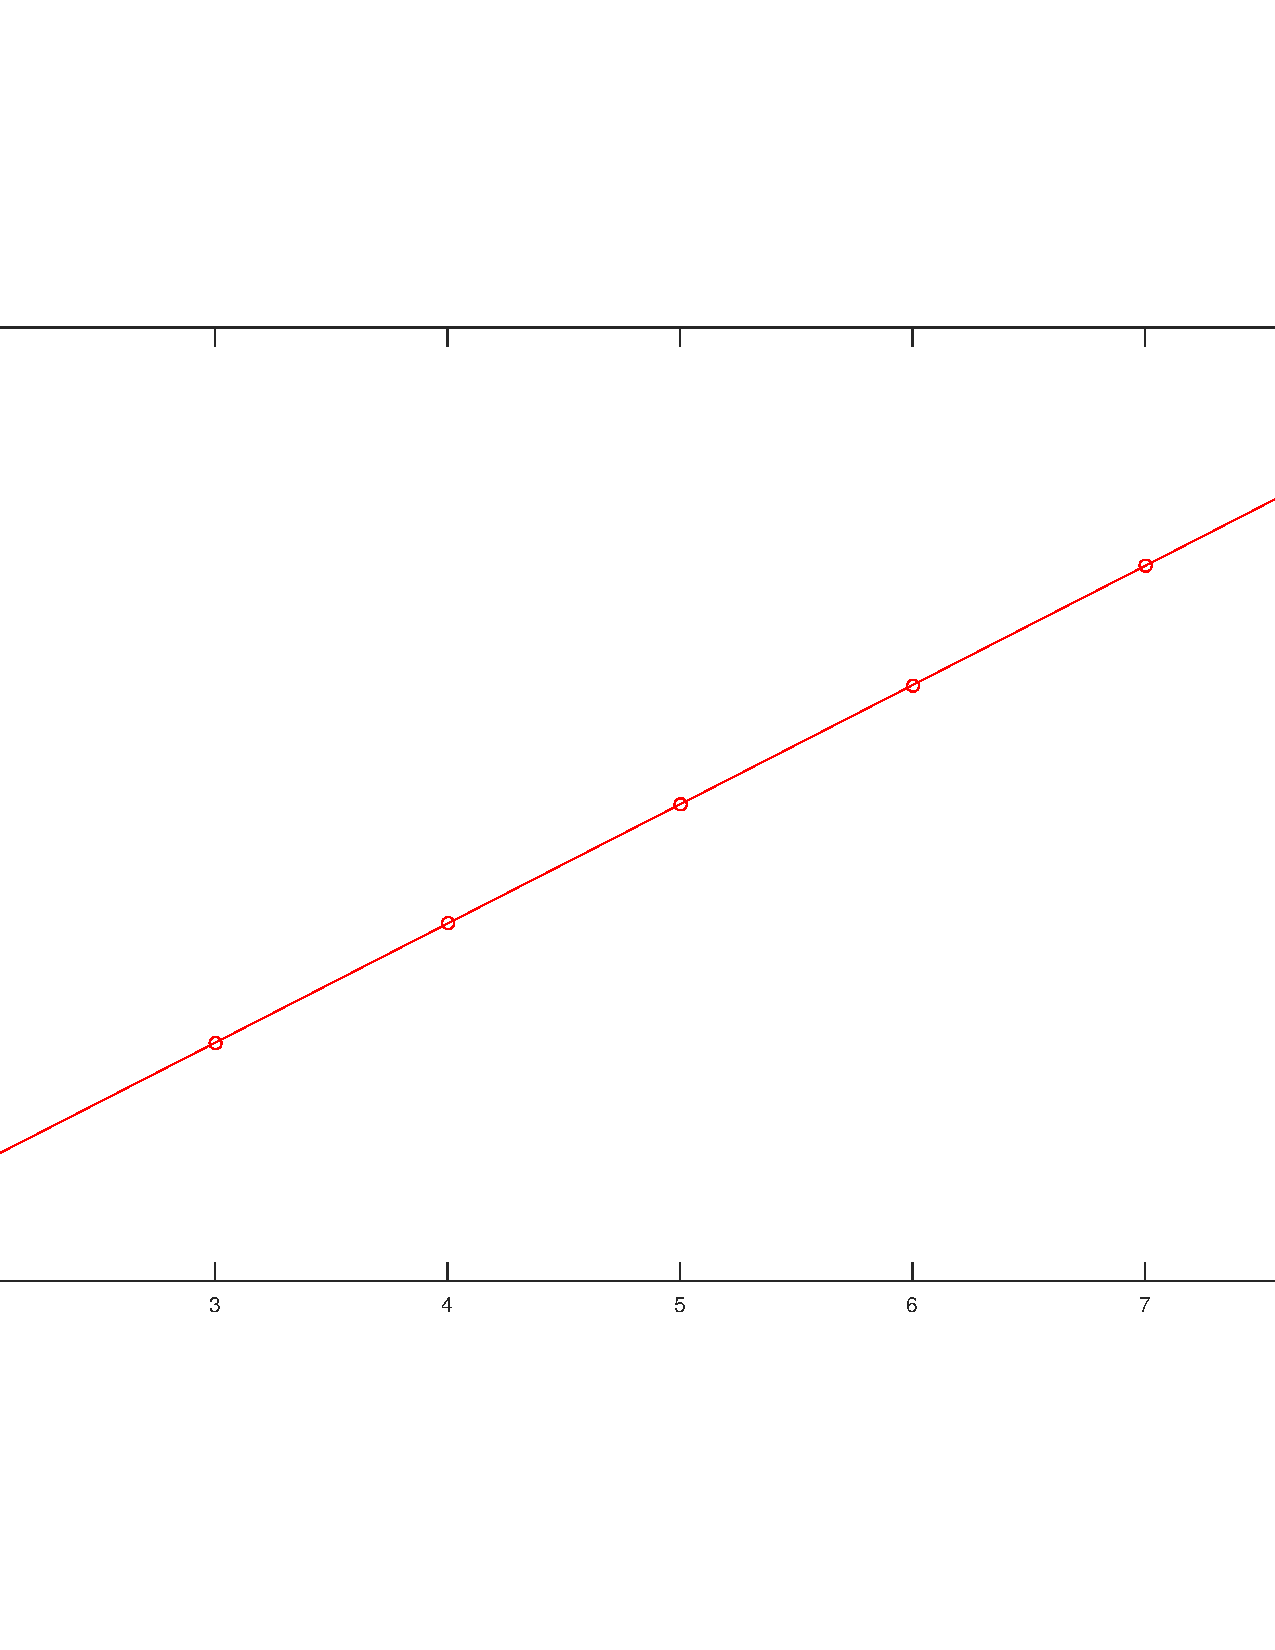
\includegraphics[width=\columnwidth]{replace_graph.pdf}}
% \caption{Plot of pneumatic cannon firing angle vs ending angle} 
% \label{fig:TradvsAutoDrop}
%\end{figure}






%
\section{Comparision}\label{sec:Comparision}


\begin{figure} \centering
  {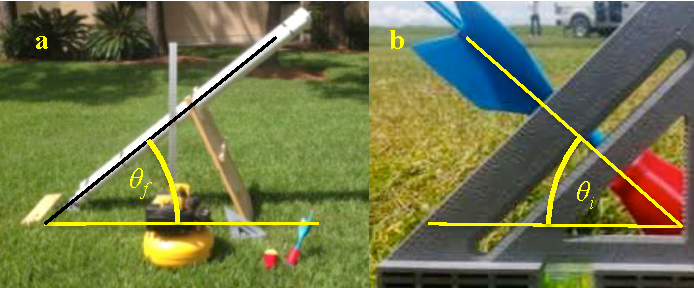
\includegraphics[width=\columnwidth]{CannonPicture}}
 \caption{A pneumatic launcher for SeismicDarts.  Ballistic dart deployment has limited usefulness because the incident angle is equal to the firing angle.} 
 \label{fig:CannonPicture}
\end{figure}

\begin{figure*}[htb]
\centering 
\vspace{1em}
\renewcommand{\figwid}{0.5\columnwidth}
\begin{overpic}[width =\figwid]{sim1_1.pdf}
\end{overpic}
\begin{overpic}[width =\figwid]{sim1_2.pdf}
\end{overpic}
\begin{overpic}[width =\figwid]{sim1_3.pdf}
\end{overpic}
\begin{overpic}[width =\figwid]{sim1_4.pdf}
\end{overpic}
\caption{Screenshots of simulations that were performed to estimate time take by different sensors surveying 100x100 m grid: a.) only SeismicSpiders b.) SeismicDarts and deployment system c.) heterogeneous system d.) human workers.
\label{fig:Sim_overview}}
\end{figure*}

\subsection{Ballistic Deployment}
To compare an alternative deployment mechanism we built the pneumatic cannon shown in Fig.~\ref{fig:CannonPicture}a.
The pneumatic cannon is U-shaped,  2 m in length, with a 0.1 m (4 inch) diameter pressure chamber and a 0.08 m (3 inch) diameter firing barrel, connected by an electronic valve (Rain Bird JTV/ASF 100). 
The cannon is aimed by selecting an appropriate firing angle $\theta_f$, azimuth angle, and chamber pressure.  
The reachable workspace is an annular ring whose radius $r$ is a function of the firing angle and initial velocity $v$. 
Neglecting air resistance, this range is found by integration:
\begin{align}
r = \frac{v^2}{g} \sin( 2 \theta_f )
\end{align} 
Initial velocity is limited by the maximum pressure and size of the pressure chamber.
The cannon used  SCH 40 PVC, which is limited to a maximum pressure of 3 Mpa (450 psi).

We charged our system to 1 Mpa (150 psi), and achieved a range of $\approx$ 150 m.
This range is considerably smaller than the UAV's range, which when loaded can complete a round trip of $\approx 1.5$ km.

A larger problem, illustrated in Fig.~\ref{fig:CannonPicture}, is that angle of incidence $\theta_i$ is equal to the firing angle $\theta_f$. 
Maximum range is achieved with $\theta_f = 45^\circ$, but this angle of incidence reduces the geophone sensitivity to $\cos(\theta_f )\approx 0.7$.
The placement accuracy of the cannon is lower than the UAV because a fired dart must fly over a longer distance than a dropped dart. 
Safety reasons also limit applications for a pneumatic launcher.





\begin{table} \centering
  {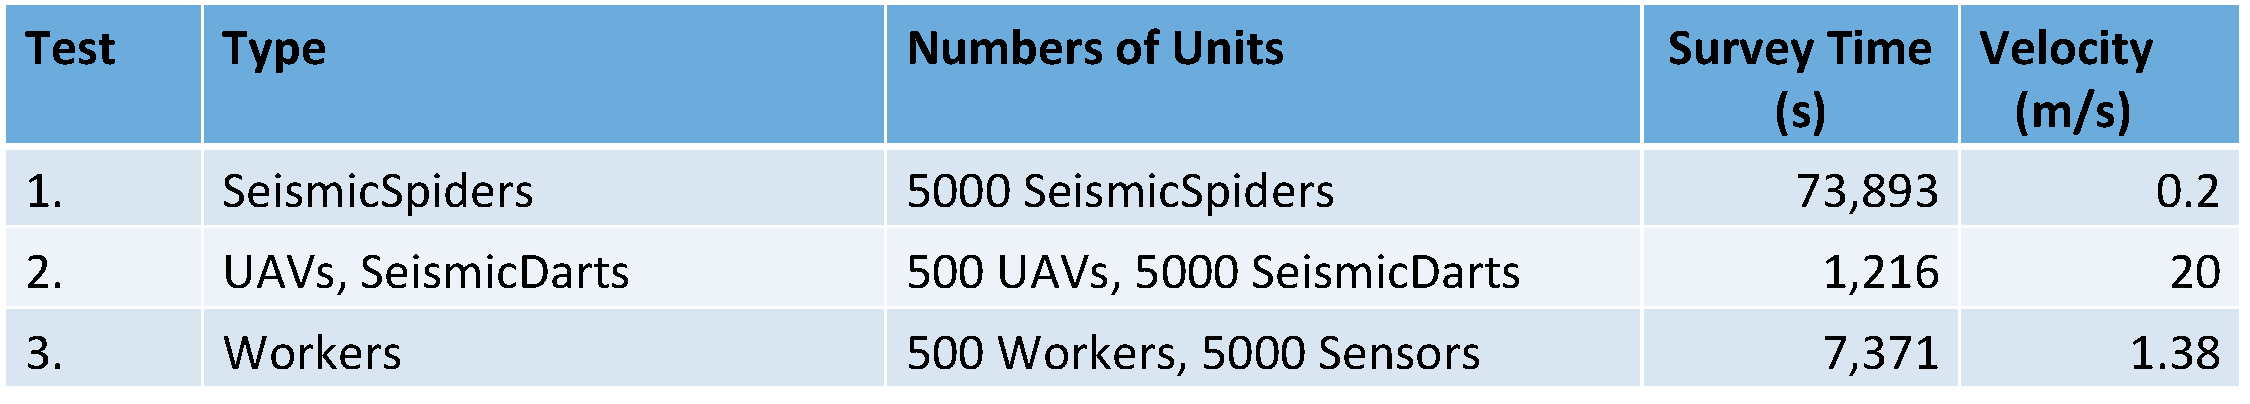
\includegraphics[width=\columnwidth]{simulation_table.pdf}}
 \caption{Comparison of different  deployment modes highlights the efficiency of UAV deployment.} 
 \label{tab:Sim_table}
\end{table}

\begin{figure} \centering
  {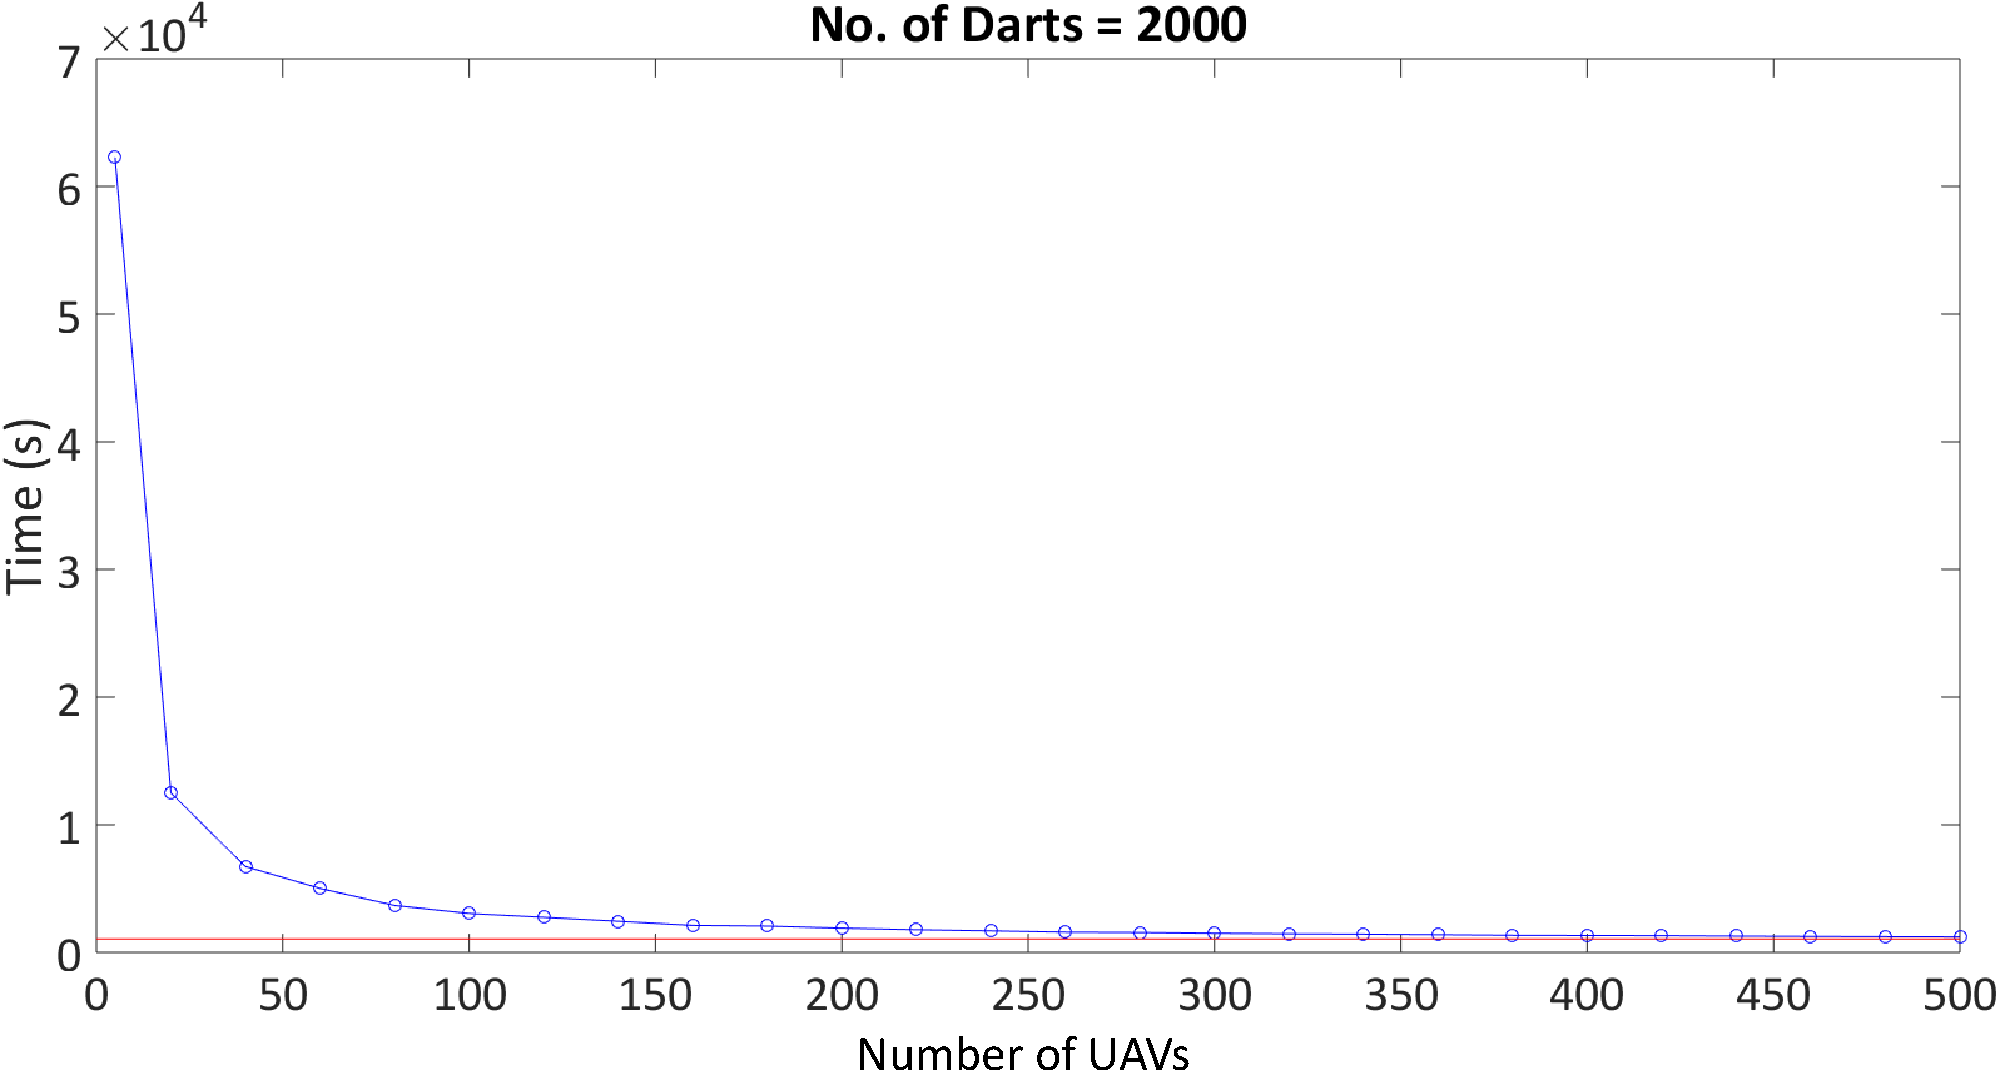
\includegraphics[width=\columnwidth]{DronevsTime.pdf}}
 \caption{Survey time for a 1km x 10 km region for different numbers of UAVs.} 
 \label{fig:DronevsTime}
 \vspace{-1em}
\end{figure}

\begin{figure} \centering
  {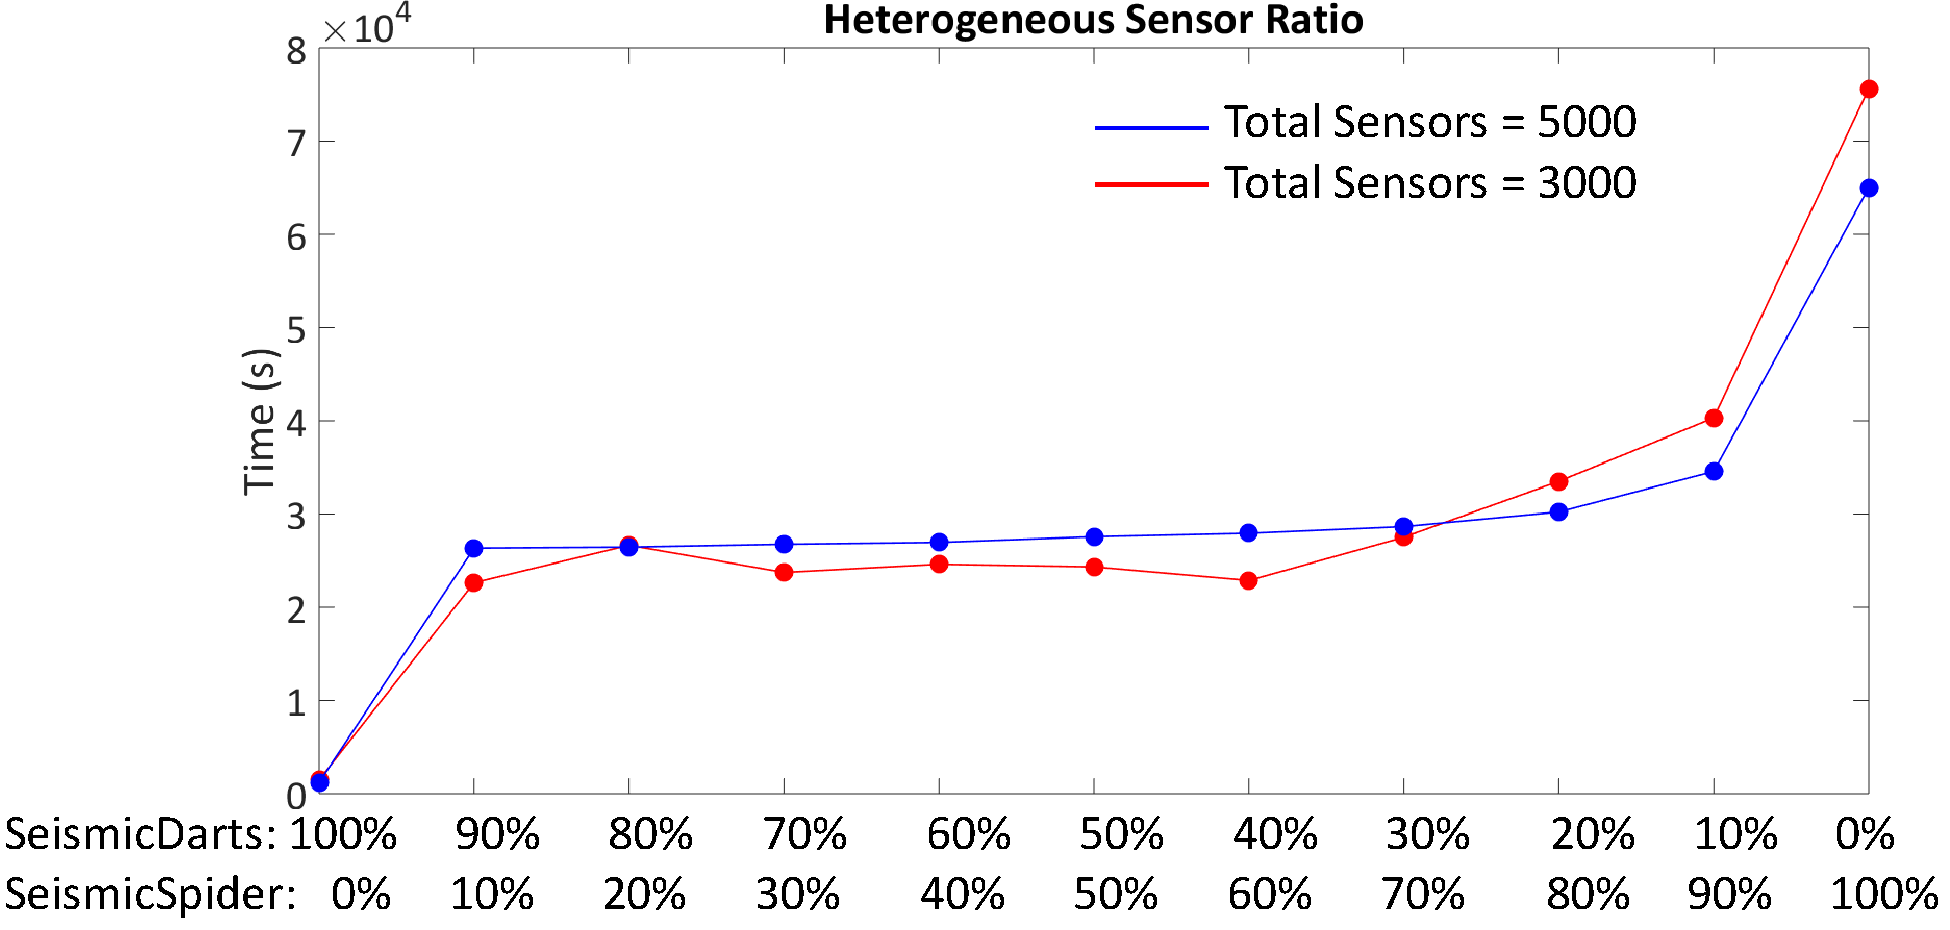
\includegraphics[width=\columnwidth]{het_sen_ratio.pdf}}
 \caption{Survey time for different sensor ratios. The total number of sensors \{5000, 3000\} were kept constant. Ten darts were provided for each UAV. } 
 \label{fig:het_sen_ratio}
  \vspace{-1em}
\end{figure}

\subsection{Simulation Studies}
   A scheduling system to compare  time and costs for seismic surveys with varying numbers of UAVs, SeismicSpiders, SeismicDarts, and human laborers was coded in  {\sc Matlab}, available at \cite{Srikanth2016seismicScheduler}.
% The goal of the Seismic Survey Scheduler is to estimate the requirements for a specific seismic survey. 
% The scheduler compare  time and costs for seismic surveys with varying numbers of UAVs, SeismicSpiders, SeismicDarts, and human laborers was coded in  {\sc Matlab}, available at \cite{Srikanth2016seismicScheduler}. 
   In each simulation, a seismic source must be measured at every survey point. 
   The scheduler must assign each sensor (SeismicDart or SeismicSpider) to an unmeasured survey point and assign each UAV or human worker a dart to pickup or deploy.  Once a sensor reaches a survey point, that sensor must wait until a seismic source is measured.
   A vibration truck (blue) provides the seismic source.
   Motion planning uses a centralized, greedy strategy.
   
   Frames from four different cases on a small survey region are shown in Fig.~\ref{fig:Sim_overview} on a 100x100 m area with survey points at 10 m spacing:
   a.) simulates 10 SeismicSpiders;  
   b.) simulates 5 SeismicUAVs deploying 50 SeismicDarts. Each UAV was allowed to carry up to 4 darts;
   c.) simulates 10 SeismicSpider, 5 SeismicUAVs and 50 SeismicDarts;
   d.) simulates 5 human workers deploying 75 SeismicDarts. Each worker was allowed to carry up to 10 darts. 
 Survey points are grey circles if unmeasured and green if measured.   The simulation uses red hexagons for SeismicSpiders,  black diamonds for UAVs,  inverted yellow triangles for SeismicDarts, and magenta diamonds for human workers. The assigned motion path for each sensor is colored magenta and the path completed is blue. 
 %The program simulates a seismic survey and records the time required. This allows comparing different combinations of sensing assets.

   
%  The first frame in Fig.~\ref{fig:Sim_overview} corresponds to SeismicSpiders (red hexagons) surveying a area of 100x100 m. 
%  Ten SeismicSpiders moving at a velocity of $0.1$m/s tries to visit each survey point (indicated by blue circles) on the map. 
%  Once ten of these sensors are at a new survey location the blue truck (Seismic source) perturbs the ground creating a seismic wave. The SeismicSpiders record the values at their current locations. 
%  Then they start moving to their next location and we repeat this process until we obtain readings at the survey locations. 
% % We follow a greedy approach to identify the SeismicSpiders new location.
%   The second frame in Fig.~\ref{fig:Sim_overview} corresponds to SeismicUAV (Black Diamond) deploying the SeismicDarts (inverted yellow triangle).
%    One SeismicUAV can carry four SeismicDarts simultaneously and drop them at different locations. 
%    Similar to the simulation involving the SeismicSpider once ten sensors are at a new survey point the blue truck takes a shot. 
%    The SeismicDarts record the readings at their corresponding locations.
%     Once this is done the SeismicUAV will pick up these SeismicDarts and redeploy them at new survey point.
%     % We follow a greedy approach to deploy these sensors. 
%      The third frame in Fig.~\ref{fig:Sim_overview} combines the SeismicSpider and SeismicDarts.
%       This represents a heterogeneous system surveying. 
%       The fourth frame in Fig.~\ref{fig:Sim_overview} represents human workers (magenta diamonds) servicing a region.
%        In all the simulations red lines connect the sensor location the sensor just surveyed to it's new location. 
%        The blue line connects the location the sensor just surveyed to it's current location. 
%        All sensors are assumed to start from the blue truck at $T = 0$. 
%        The Seismic Survey  simulates the proposed system and comparison with manual deployment could be achieved for analysis. 
%        The simulator is robust and all the parameters described above are variables. 
%        We want this tool to be used for preprocessing of a seismic survey in which you can vary the number of sensors, velocity, size of seismic survey, location of the seismic source etc.
%         Using this simulator we can closely match a real seismic survey and thus optimize the resources.
 

%A scheduling system to compare  time and costs for seismic surveys with varying numbers of UAVs, SeismicSpiders, SeismicDarts, and human laborers was coded in  {\sc Matlab}, available at \cite{Srikanth2016seismicScheduler}. Frames from four different cases are shown in Fig.~\ref{fig:Sim_overview}.

This tool allows us to examine engineering and logistic trade-offs quickly through simulations.  For example, Fig.~\ref{fig:DronevsTime} assumes a fixed number of darts and examines the finishing time with $5$ to $500$ UAVs.  The time required decays asymptotically, but $140$ UAVs requires only twice the amount of time required for $500$ UAVs, indicating  $140$ UAVs are sufficient for the task.    
 Substantial cost savings can be obtained by selecting the number of UAVs required to complete within a certain percentage greater than the optimal time.

The tool is useful for comparing the effectiveness of heterogeneous teams.  Table~\ref{tab:Sim_table} compares surveying a $1$ km x $10$ km strip of land with teams of (a) $5000$ SeismicSpiders, (b) $500$ UAVs and $5000$ SeismicDarts, (c) $500$ humans and $5000$ geophones.  Team (b) completed six times faster than team (c). 
  Since SeismicSpiders are  slower than UAVs and humans and are expensive compared to the SeismicDarts, their use is limited to special occasions. The UAV can deploy the SeismicSpider at a given waypoint. This attribute was not considered in the simulation but would improve deployment speed of SeismicSpiders.
   
In Fig.~\ref{fig:het_sen_ratio}, the total number of mobile agents are constant, but the percentage of UAVs and SeismicSpiders are varied.  10 SeismicDarts were provided for each UAV. Increasing the percentage of UAVs lowers the deployment time because UAVs move 20 m/s but SeismicSpiders move 0.2 m/s. 
The velocity difference makes UAV deployment time-efficient. 

%
% Thesis 

\chapter[Conclusion]{Conclusion}
\label{chap-conc}

In this thesis, three applications for autonomous unmanned vehicles were presented.
Unmanned aerial vehicles (UAV) can be used to deploy, retrieve geophones for seismic surveying and deploy unmanned rover attached with geophones.
We presented software to plan for a wireless sensor network deployment using UAV and unmanned rover.
A UAV was used to drag an electrified net through an area to destructively survey mosquito populations.
We used our collaborator's algorithm to reduce the energy expenditure while maximizing area covered.
An updated design for drifting wireless sensor node was presented.
The drift node can be used to survey coastlines and national maritime boundaries for marine border security, wildlife science missions.

In future work, the applications above could be merged together for a more complete package.
A wireless sensor network can then be deployed, monitored and retrieved by AUVs.
Before the WSN deployment, the area can be surveyed by a UAV with minimal energy expenditure.
Wireless sensor nodes can communicate with each other to relay position, cache data or relay data back to the base station.
Like in \cite{sudarshanwsn}, UAVs can monitor data and charge wireless sensor nodes, extending their longevity.
For destructive mosquito surveying methods, the UAVs can incorporate live data to plan its route reactively.

%We developed a method to deploy geophones for seismic surveying with AUVs, reducing manual labors and injury risks.
%The geophones are combined with a data recording unit, can record its own position and the soundwave during the seismic survey.
%This eliminate long analog data transmisison cables, which reduce a large part of equipment weight during surveying.
%We can drop geophones from our UAVs when we put the geophones a SeismicDart shell, which eliminates the need for a separate UAV per sensor.
%For terrains that UAVs cannot fly to or the SeismicDart cannot approach, we developed a SeismicSpider, with geophones for legs.
%The SeismicSpider can travel to its desired position, with geohphones contacting the ground, record the soundwave during the survey.
%The software we developed to schedule a seismic survey can be used for many other wireless sensor network applications that use UAVs and autonomous rovers.



\bibliographystyle{IEEEtran}
\bibliography{./bibs/match}

% that's all folks
\end{document}


